% Reference document for the final report (Milestone 10).
% This is NOT the final report. It collects the facts, equations, numbers, tables, figures and
% citations the author needs to write the report. Every number traces to a run folder under
% results/ or to IMPLEMENTATION_LOG.md. Build: pdflatex reference && bibtex reference &&
% pdflatex reference && pdflatex reference (or upload the report/ folder to Overleaf).
\documentclass[11pt,a4paper]{article}

\usepackage[utf8]{inputenc}
\usepackage[T1]{fontenc}
\usepackage[margin=2.2cm]{geometry}
\usepackage{amsmath,amssymb}
\usepackage{booktabs}
\usepackage{tabularx}
\usepackage{graphicx}
\usepackage{xcolor}
\usepackage{enumitem}
\usepackage{url}
\usepackage[authoryear,round]{natbib}
\usepackage[colorlinks=true,linkcolor=blue!50!black,citecolor=green!35!black,urlcolor=blue!50!black]{hyperref}

\graphicspath{{figures/}}
\setlist{itemsep=2pt,topsep=4pt}

% Status tags. Use them to keep implemented, measured, exploratory and pending items apart.
\newcommand{\statustag}[2]{\colorbox{#1}{\scriptsize\sffamily\bfseries #2}}
\newcommand{\implemented}{\statustag{blue!12}{IMPLEMENTED + TESTED}}
\newcommand{\confirmatory}{\statustag{green!18}{CONFIRMATORY, EVALUATION SEEDS}}
\newcommand{\exploratory}{\statustag{orange!20}{EXPLORATORY}}
\newcommand{\tuning}{\statustag{gray!20}{TUNING SEEDS ONLY}}
\newcommand{\pending}{\statustag{red!15}{PENDING}}
\newcommand{\src}[1]{{\footnotesize\textit{Source:} \path{#1}}}

\newcommand{\zhat}{\hat{z}}
\newcommand{\TV}{\operatorname{TV}}
\newcommand{\NDCG}{\mathrm{NDCG}}

\title{Adaptive Interest-Weighted Diversification for Session-Based Recommendation under Dynamic User Intent\\[4pt]
\large Reference document for the final report (not the report itself)}
\author{Shambo Roy \\ IRE course project, IIIT Hyderabad}
\date{Compiled 3 November 2026, after Milestone 9 (commit \texttt{d1822a3})}

\begin{document}
\maketitle

\begin{abstract}
\noindent This document gathers everything the final report needs: the research question,
the simulator, the methods with their equations, the evaluation protocol, all measured
results with confidence intervals, the exploratory follow-ups, negative results,
limitations, reproducibility details, a claim-to-evidence map and viva notes. It is written
as reference material rather than polished prose. Tags mark the status of each item, and all
results apply to this simulation only.
\end{abstract}

\paragraph{Status tags.}
\implemented\ code exists and the test suite covers it;
\confirmatory\ the single frozen run on seeds 100--119;
\exploratory\ follow-ups on seeds 200--219, decided after seeing confirmatory results;
\tuning\ design and tuning evidence on seeds 0--4;
\pending\ not done yet.

\tableofcontents
\newpage

%=====================================================================================
\section{Research question and contribution}
%=====================================================================================

\paragraph{Central question.} Can adaptive estimation of a user's changing category
interests, combined with interest-weighted DPP selection, improve the balance of relevance,
diversity and responsiveness to changing intent, compared with non-adaptive and non-DPP
baselines?

\begin{itemize}
  \item \textbf{RQ1 (adaptation).} Does an adaptive estimator track the true interest $z_t$
        better after drift, and at what cost when interests are stable or clicks are noisy?
  \item \textbf{RQ2 (diversification).} How much does DPP selection gain in diversity, and lose in
        relevance, for focused and for spread interests?
  \item \textbf{RQ3 (interaction).} Do adaptation and DPP diversification complement or
        substitute for each other?
\end{itemize}

\paragraph{Approach.} A controlled, open-loop simulation in which the true latent interest
$z_t$ is known. A $2\times 2$ factorial design crosses the profile (static cumulative mean vs
adaptive bias-corrected EWMA) with the selector (Top-$K$ vs greedy DPP), across five drift
scenarios and two interest-concentration levels. Popularity and oracle-$z$ methods serve as a
floor and a diagnostic ceiling.

\paragraph{What the contribution is, and is not.}
\begin{itemize}
  \item \textbf{No novelty claim for the method.} Personalised quality inside a DPP kernel
        \citep{ibrahim2025personalized}, DPP kernels adapted over interactions
        \citep{liu2019d2rl}, personalised diversification \citep{teo2016adaptive} and
        exponential forgetting of history \citep{ding2005time,koren2009temporal} already exist.
  \item \textbf{The contribution is a controlled empirical analysis.} It measures estimation
        error and adaptation lag against ground truth, and it separates the adaptation and
        selection effects and their interaction across drift types and concentrations. In the
        sources we reviewed (30, a targeted search rather than a systematic review), we did not
        find such a study. ``Not found'' does not mean ``does not exist''.
  \item \textbf{External validity is limited.} The results are synthetic and do not show
        real-world effectiveness \citep{stavinova2022synthetic}.
\end{itemize}

%=====================================================================================
\section{Related work: what each source supports}
%=====================================================================================
Verification levels are recorded in \path{literature/literature_matrix.md}. Most entries are
checked at the metadata and abstract level only. Cite them only for claims that level
supports.

\begin{description}[style=nextline]
  \item[DPPs] $P(Y)\propto\det L_Y$; the L-ensemble $L=\mathrm{Diag}(q)\,S\,\mathrm{Diag}(q)$ splits
        into quality and diversity \citep{kulesza2012dpp}. Fixed-size $k$-DPPs exist
        \citep{kulesza2011kdpp}. MAP is NP-hard \citep{ko1995exact} and hard to approximate
        (Kulesza \& Taskar, Thm 2.9, read in full). Better-than-greedy MAP methods exist
        \citep{gillenwater2012map}.
  \item[DPP recommendation] Fast greedy MAP with incremental Cholesky updates and a
        relevance--diversity trade-off \citep{chen2018fast}, our algorithm. Industrial DPP
        re-ranking \citep{wilhelm2018youtube}. DPP likelihoods for sequential models
        \citep{liu2022dppseq}. RL-adapted kernels \citep{liu2019d2rl}. A personalised DPP whose
        online deployment reduced click-through rate \citep{ibrahim2025personalized}: a warning
        that diversity can cost relevance.
  \item[Diversity and intent] MMR \citep{carbonell1998mmr}; topic diversification and
        intra-list similarity, where accuracy fell but satisfaction rose
        \citep{ziegler2005topic}; intent-aware search diversification
        \citep{agrawal2009diversifying}; novelty and diversity evaluation
        \citep{clarke2008novelty}; intent-oriented recommendation diversity
        \citep{vargas2011intent}; surveys \citep{kaminskas2016diversity,wu2024diversification}.
  \item[Calibration] Matching list composition to a user's genre distribution
        \citep{steck2018calibrated}, read in full on 3 November 2026 and used as a
        baseline (\S\ref{sec:calib}). Calibrating against recent windows instead of the full history
        \citep{lin2024beyond}, conceptually the closest work: static vs time-windowed profiles,
        but with calibration rather than a DPP, and on real data without ground truth.
  \item[Session-based] GRU4Rec \citep{hidasi2016gru4rec}; simple heuristics are often
        competitive \citep{ludewig2018evaluation}, which supports a transparent base scorer;
        survey \citep{wang2021survey}; multi-interest models with an accuracy--diversity factor
        \citep{cen2020comirec}.
  \item[Drift] Vocabulary for sudden, gradual and recurring drift, and forgetting by fading
        factors and windows \citep{gama2014survey}; adaptive windows \citep{bifet2007adwin}.
  \item[Simulation] Latent-state user simulators as a research tool \citep{ie2019recsim}; the
        gap between simulated and real behaviour \citep{stavinova2022synthetic}.
\end{description}

%=====================================================================================
\section{Simulator}\label{sec:sim}
%=====================================================================================
\implemented\ Specification: \path{SIMULATION_DESIGN.md}. Code: \path{adaptdiv/catalogue.py},
\path{scenarios.py}, \path{simulator.py}, \path{seeding.py}, \path{config.py}.

\subsection{Catalogue}
$C=10$ categories with $n_c=50$ items each ($N=500$). Centroids $\mu_c=\mathrm{normalise}(h_c)$
with $h_c\sim\mathcal N(0,I_d)$, $d=32$. Item embeddings
$\phi_i=\mathrm{normalise}(\mu_{c_i}+\sigma\varepsilon_i)$, $\varepsilon_i\sim\mathcal N(0,I_d/d)$,
$\sigma=1$. The mean cosine similarity is $0.50$ within a category and about $0$ across
categories. Popularity is $\pi_i\propto\exp(s_{\mathrm{pop}}\zeta_i)$ with $\zeta_i\sim\mathcal N(0,1)$,
$s_{\mathrm{pop}}=1$, normalised within each category. The catalogue is regenerated for every
seed.

\subsection{Latent interests and drift}
$z_t\in\Delta^{C-1}$. Base interest $z_A\sim\mathrm{Dirichlet}(\kappa\mathbf 1_C)$ with
$\kappa\in\{0.1\ \text{(focused)},\,1.0\ \text{(spread)}\}$. The expected largest component is
0.67 and 0.29 respectively, and about 2.0 and 5.2 categories hold 80\% of the mass. The shifted
interest $z_B=Pz_A$ uses a half-swap permutation: the top $C/2$ categories map onto the bottom
$C/2$ and vice versa. The mean $\TV(z_A,z_B)$ is 0.99 (focused) and 0.64 (spread), and
concentration is unchanged by the shift.

\begin{table}[h]\centering\small
\begin{tabular}{lll}
\toprule
Scenario & Trajectory ($T=200$) & Used by \\
\midrule
Stable    & $z_t=z_A$ & H2, H4b \\
Abrupt    & $z_A$ for $t<100$, then $z_B$ & H1, H4a, H6 \\
Gradual   & $(1-w_t)z_A+w_tz_B$, $w_t=\mathrm{clip}((t-80)/40,0,1)$ & H1, H4a, H6 \\
Recurrent & $z_A$, then $z_B$ from $t=70$, back to $z_A$ from $t=140$ & H1, H4a, H6 \\
Noisy     & $z_t=z_A$, click noise $\eta=0.3$ & H3 \\
\bottomrule
\end{tabular}
\caption{Drift scenarios. Shift times are fixed so that post-shift windows line up across users.}
\end{table}

\subsection{Interaction model}
At each step: a noise flag $n_t\sim\mathrm{Bernoulli}(\eta)$ with $\eta=0.05$ (0.3 in the noisy
scenario); category $c_t\sim\mathrm{Cat}(z_t)$ if $n_t=0$, otherwise uniform; then item
$P(i\mid c,u)\propto\pi_i^{\gamma}\exp(\lambda\,\hat s_i(u))$ within the category, where $u$ is a
hidden taste vector, $\hat s_i(u)$ the standardised $\langle\phi_i,u\rangle$, $\gamma=1$,
$\lambda=0.5$. Repeats are allowed. The exact marginal is
\begin{equation}
P_t(i)=\big[(1-\eta)z_{t,c_i}+\eta/C\big]\;P(i\mid c_i,u).
\end{equation}
The hidden taste ($\lambda>0$) is information the recommender cannot model, so even the oracle
is not right by construction. Observed categories follow $(1-\eta)z_t+\eta/C$, which creates a
noise floor $\TV=\eta\,\TV(z_t,\mathrm{uniform})$ for any tracker.

\subsection{Leakage firewall and seeds}
The simulator returns an \texttt{ObservedSequence} (item ids only) and a separate
\texttt{GroundTruth}. Estimators and recommenders see only observed items, public item
categories and embeddings, and popularity estimated from a separate training population of
1{,}000 users $\times$ 50 interactions per seed. A test checks that the observed type carries
no ground-truth field. Seeds come from \texttt{SeedSequence} streams keyed by (seed, path).
Scenarios reuse each user's random-number bank (common random numbers), so scenario
comparisons are paired, and before the first switch the stable, abrupt and recurrent
sequences are identical.

\paragraph{Seed sets.} Tuning 0--4; evaluation 100--119 (used once, at Milestone 8);
exploratory 200--219 (Milestone 9). Scale per seed: 2 $\kappa$ $\times$ 5 scenarios $\times$
100 users $\times$ 200 steps $=200{,}000$ interactions.

\begin{figure}[h]\centering
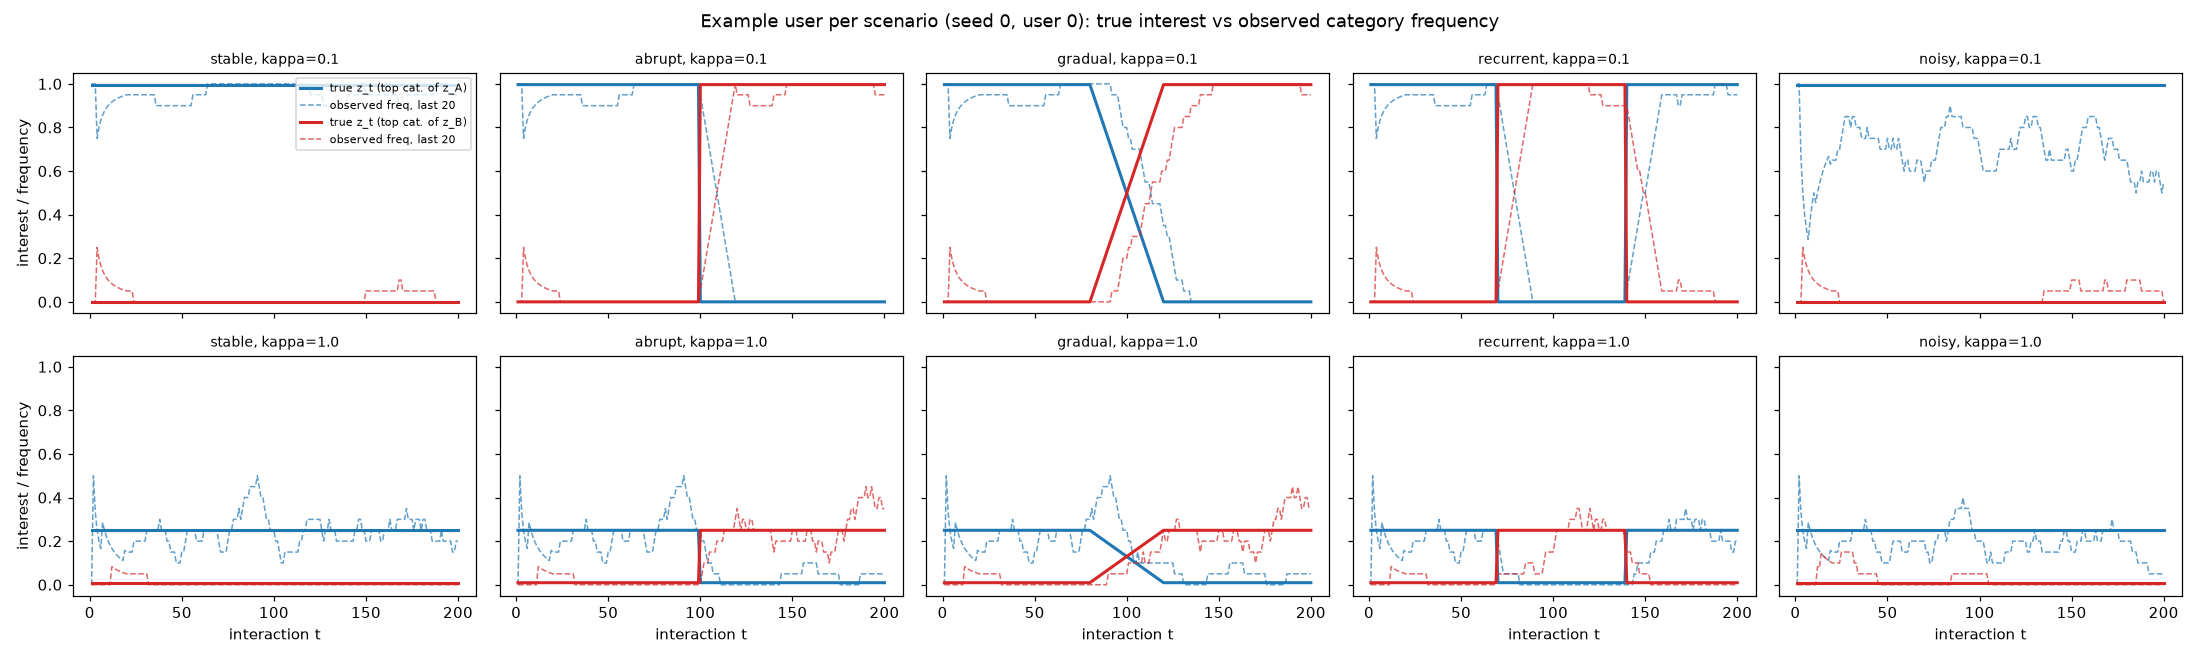
\includegraphics[width=\linewidth]{m3_trajectories.png}
\caption[Example trajectories]{One example user per scenario and concentration: true $z_t$ for the top categories
of $z_A$ and $z_B$ against the rolling 20-interaction observed frequency. \tuning\
\src{results/m3_sim_check/20261026-192349/}}
\end{figure}

%=====================================================================================
\section{Methods}\label{sec:methods}
%=====================================================================================
\implemented\ Code: \path{adaptdiv/estimators.py}, \path{relevance.py}, \path{similarity.py},
\path{dpp.py}, \path{recommenders.py}.

\subsection{Interest estimators}
With $x_t=e_{c_{i_t}}$, the one-hot category of the observed item:
\begin{align}
\text{Cumulative mean (static):}\quad & \zhat_t=\tfrac1t\textstyle\sum_{s\le t}x_s,\\
\text{Bias-corrected EWMA (adaptive):}\quad & m_t=(1-\alpha)m_{t-1}+\alpha x_t,\ m_0=0,\quad \zhat_t=\frac{m_t}{1-(1-\alpha)^t},\\
\text{Uniform-start EWMA (ablation):}\quad & \zhat_t=(1-\alpha)\zhat_{t-1}+\alpha x_t,\ \zhat_0=\mathbf 1/C,\\
\text{Sliding window (ablation):}\quad & \zhat_t=\tfrac{1}{\min(t,W)}\textstyle\sum_{s=\max(1,t-W+1)}^{t}x_s.
\end{align}
EWMA weights decay geometrically, with mean observation age $(1-\alpha)/\alpha$; a window has
the same mean age when $W\approx 2/\alpha-1$. The bias correction removes the uniform prior's
influence on early estimates (D-27). Selected values: $\alpha=0.05$ for the proposed estimator
and $\alpha=0.07$ for the uniform-start ablation, each tuned for tracking error on tuning
seeds; $W=40$.

\subsection{Scores, similarity and selection}
Base relevance is within-category popularity from the training population,
$r_i=(\mathrm{count}_i+1)/(\sum_{j\in c_i}\mathrm{count}_j+n_c)$. The score is
\begin{equation}
s_i(t)=r_i\,\big(\zhat_{t,c_i}+\epsilon\big),\qquad \epsilon=0.01,
\end{equation}
and the similarity kernel is $S=\Phi\Phi^\top+10^{-6}I$. All $N$ items are candidates, and the
list for step $t+1$ uses $\zhat_t$ only. The selection objective, our adaptation of
\citet{chen2018fast} (D-14), is
\begin{equation}
F(Y)=\theta\sum_{i\in Y}\log s_i+(1-\theta)\log\det S_Y,\qquad |Y|=K=10.
\end{equation}
For $\theta<1$ this equals $(1-\theta)\log\det L_Y$ with
$L=\mathrm{Diag}(q)\,S\,\mathrm{Diag}(q)$, $q_i=s_i^{\theta/(2(1-\theta))}$, so it is a valid DPP
with log-linear quality. $\theta=1$ is exactly Top-$K$, which puts both selectors on one
scale. \textbf{Report wording:} Chen et al.\ use a linear form $\theta\sum r_i$. It failed at
our score scale, so the log form is our adaptation and their results do not transfer
directly.

\paragraph{Greedy MAP} (Chen et al., Algorithm 1). Keep $c_i$ and $d_i^2$; repeatedly pick
$j=\arg\max_i\,\theta\log s_i+(1-\theta)\log d_i^2$, then update
$e_i=(S_{ji}-\langle c_j,c_i\rangle)/d_j$, append $e_i$ to $c_i$ and set
$d_i^2\leftarrow d_i^2-e_i^2$. The cost is $O(K^2N)$, measured at 0.12--0.18\,ms per list.
Greedy matched the exact optimum on 95\%, 99.5\% and 100\% of 200 tiny instances (14 items,
$k=5$) at $\theta=0.3,0.6,0.8$. This is tested on tiny instances only and does not bound the
gap at $N=500$. Call it \emph{greedy approximate MAP}. DPP lists are sorted by score before
evaluation, so both selectors use the same ranking rule.

\begin{table}[h]\centering\small
\begin{tabular}{lll}
\toprule
Method & Profile & Selector \\
\midrule
Popularity & none (global popularity) & Top-$K$ \\
Static Top-$K$ / Static DPP & cumulative mean & Top-$K$ / DPP $\theta=0.5$ \\
Adaptive Top-$K$ / Adaptive DPP & bias-corrected EWMA, $\alpha=0.05$ & Top-$K$ / DPP $\theta=0.5$ \\
Oracle Top-$K$ / Oracle DPP (diagnostic) & true $z_{t+1}$ & Top-$K$ / DPP $\theta=0.5$ \\
Ablations & uniform-start EWMA ($\alpha=0.07$); window ($W=40$) & both \\
Calibrated (M10, exploratory) & static or adaptive & Steck-style re-ranker, $\lambda=0.8$ (\S\ref{sec:calib}) \\
\bottomrule
\end{tabular}
\caption{Methods (D-16). Oracles are ceilings, excluded from H6a.}
\end{table}

%=====================================================================================
\section{Evaluation protocol}\label{sec:eval}
%=====================================================================================
\implemented\ Code: \path{adaptdiv/metrics.py}, \path{evaluation.py}, \path{stats.py},
\path{confirmatory.py}. Decisions D-17, D-21, D-29, D-30.

\subsection{Metrics}
$R_t$ is the list built from $\zhat_t$, and $T_t$ is the set of distinct items among the next
$h=5$ clicks. Lists are scored for $t=20,\dots,T-h$.
\begin{itemize}
  \item \textbf{NDCG@10} (primary relevance): binary gain,
        $\sum_{p=1}^{K}\mathbf 1[R_t(p)\in T_t]/\log_2(p+1)$, divided by the ideal for
        $\min(|T_t|,K)$ hits.
  \item Recall@10; \textbf{expected utility} EU@10 $=\sum_{i\in R_t}P_{t+1}(i)$, computed by
        the simulator and used for the $\theta$ rule; new-item NDCG and EU as a sensitivity
        check on repeats.
  \item \textbf{Category coverage} (primary diversity): distinct categories in $R_t$ divided by
        $\min(K,C)$. ILD, the mean pairwise $1-\cos$, is descriptive only, because the DPP
        optimises it directly. Seen share is the fraction of $R_t$ already clicked.
  \item \textbf{Estimation:} tracking error $\TV(\zhat_t,z_t)$; crossover lag, the first $L$
        such that $\zhat$ is closer to the new interest than to the old one for 5 consecutive
        steps, censored at the horizon; false-switch rate, the share of steps where
        $\arg\max\zhat$ changes while $\arg\max z$ does not.
\end{itemize}
The post-shift window is the 50 steps from each switch (abrupt 100, gradual midpoint 100,
recurrent 70 and 140). Values are aggregated step $\to$ user $\to$ cell $\to$ seed.
``Drift pooled'' means the equal-weight mean over abrupt, gradual and recurrent and both
$\kappa$.

\subsection{Statistics and freeze}
The unit of analysis is the seed-level mean, paired across methods (20 seeds). Tests are
two-sided Wilcoxon signed-rank (smallest possible $p=1.91\times10^{-6}$), with a percentile
paired bootstrap 95\% CI and Holm correction over 8 tests. SESOI: 3\% relative for NDCG and EU,
2 interactions for lag, 0.02 for TV. ``Practically meaningful'' means the whole CI lies beyond
the SESOI. Hypotheses, metrics, SESOI, $\alpha$ and $\theta$ were \textbf{frozen on 1 November
2026}, before any evaluation seed ran (\path{hypothesis.md}).

\begin{table}[h]\centering\small
\begin{tabularx}{\linewidth}{lX}
\toprule
Test & Quantity (data) \\
\midrule
H1a & crossover lag, cumulative $-$ EWMA (drift pooled) \\
H1b & post-shift TV, cumulative $-$ EWMA (drift pooled) \\
H2 & TV, EWMA $-$ cumulative (stable, $t>20$) \\
H3 & false-switch rate, EWMA $-$ cumulative (noisy) \\
H4a & post-shift NDCG, Adaptive Top-$K$ $-$ Static Top-$K$ (drift pooled) \\
H5a & coverage, Adaptive DPP $-$ Adaptive Top-$K$ (all scenarios) \\
H5b & relative NDCG cost of DPP (adaptive), focused $-$ spread \\
H6b & $(\text{AdaDPP}-\text{StatDPP})-(\text{AdaTop}-\text{StatTop})$ on post-shift NDCG, two-sided \\
\midrule
H4b (outside Holm) & equivalence: whole CI of stable relative NDCG difference within $\pm3\%$ \\
H6a (outside Holm) & Adaptive DPP not dominated on (post-shift NDCG, coverage) by Popularity, Static Top-$K$, Adaptive Top-$K$ or Static DPP \\
\bottomrule
\end{tabularx}
\caption{Confirmatory tests (D-30).}
\end{table}

%=====================================================================================
\section{Tuning on tuning seeds}\label{sec:tuning}
%=====================================================================================
\tuning

\paragraph{$\alpha$ for the estimator} (pooled mean TV over all scenarios and both $\kappa$;
\path{results/m4_ewma_init/20261101-140141/}):

\begin{table}[h]\centering\small
\begin{tabular}{lccccccccc}
\toprule
$\alpha$ & 0.02 & 0.03 & 0.05 & 0.07 & 0.1 & 0.15 & 0.2 & 0.3 & 0.5 \\
\midrule
Uniform start  & .2818 & .2474 & .2230 & \textbf{.2216} & .2330 & .2612 & .2906 & .3452 & .4384 \\
Bias-corrected & .2339 & .2210 & \textbf{.2138} & .2187 & .2339 & .2640 & .2937 & .3480 & .4402 \\
\bottomrule
\end{tabular}
\caption{Pooled tracking error. Cumulative mean: 0.2808. Best window $W=40$: 0.2164.}
\end{table}

\paragraph{$\theta$ for the DPP} (D-29: the smallest $\theta$ with EU@10 loss $\le 3\%$ against
same-profile Top-$K$, for both profiles; \path{results/m7_theta/20261101-152049/}):

\begin{table}[h]\centering\small
\begin{tabular}{lcccccc}
\toprule
$\theta$ & 0.9 & 0.8 & 0.7 & 0.6 & \textbf{0.5} & 0.3 \\
\midrule
Static EU loss   & $-0.2\%$ & $-0.3\%$ & $-0.3\%$ & 0.2\% & 1.0\% & 6.9\% \\
Adaptive EU loss & 0.0\% & 0.1\% & 0.5\% & 1.3\% & 2.8\% & 10.3\% \\
Adaptive coverage & 0.332 & 0.345 & 0.360 & 0.380 & 0.406 & 0.490 \\
\bottomrule
\end{tabular}
\caption{$\theta=0.5$ selected; it sits close to the 3\% limit.}
\end{table}

\begin{figure}[h]\centering
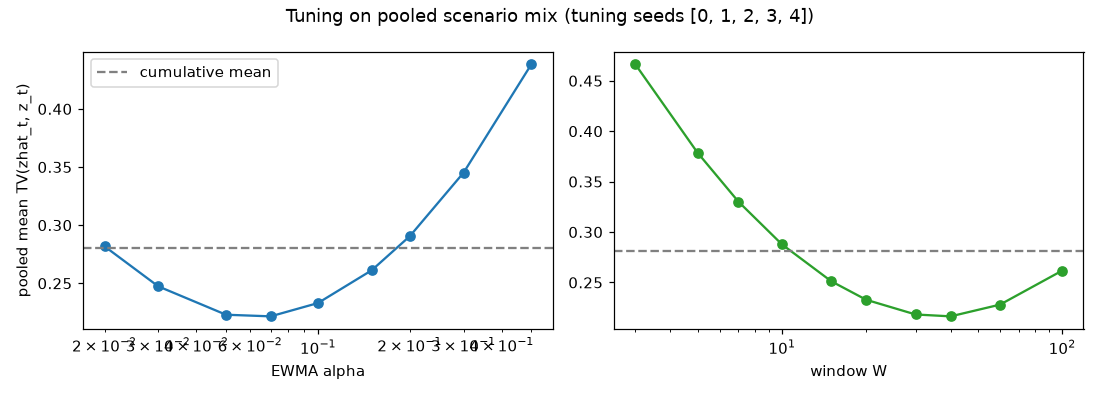
\includegraphics[width=0.9\linewidth]{m4_tuning_curves.png}
\caption[Estimator tuning curves]{Estimator tuning curves (uniform-start EWMA and windows; the bias-corrected curve is
in the table above). \tuning\ \src{results/m4_estimators/20261028-121944/}}
\end{figure}

%=====================================================================================
\section{Confirmatory results (Milestone 8)}\label{sec:m8}
%=====================================================================================
\confirmatory\ Run \path{results/m8_main/20261102-112410/}: seeds 100--119, every step, 812\,s
with 5 processes, git HEAD \texttt{f0fc858}, 29{,}440 records, no NaN. This was the first and
only run on these seeds. Seed 100 rerun alone gave all 1{,}472 values identical.

\begin{table}[h]\centering\small
\begin{tabular}{llcll}
\toprule
Test & Mean difference & 95\% CI & Holm $p$ & Verdict \\
\midrule
H1a & $+67.3$ steps & [67.0, 67.6] & $1.5\times10^{-5}$ & Supported, beyond SESOI \\
H1b & $+0.248$ TV & [0.247, 0.249] & $1.5\times10^{-5}$ & Supported, beyond SESOI \\
H2  & $+0.045$ TV & [0.045, 0.046] & $1.5\times10^{-5}$ & Supported, beyond SESOI \\
H3  & $+0.057$ & [0.055, 0.058] & $1.5\times10^{-5}$ & Supported \\
H4a & $+0.101$ NDCG ($+131\%$) & [122\%, 140\%] & $1.5\times10^{-5}$ & Supported, beyond SESOI \\
H5a & $+0.089$ coverage & [0.086, 0.092] & $1.5\times10^{-5}$ & Supported \\
H5b & $+0.0038$ & [0.0012, 0.0064] & 0.024 & Supported, very small \\
H6b & $-0.0106$ NDCG & [$-0.0111$, $-0.0100$] & $1.5\times10^{-5}$ & Significant: substitution \\
\midrule
H4b & $\approx-1.8\%$ & [$-1.9\%$, $-1.6\%$] & -- & Equivalent within $\pm3\%$ \\
H6a & -- & -- & -- & Not dominated \\
\bottomrule
\end{tabular}
\caption{Confirmatory tests. $1.5\times10^{-5}$ is the floor after Holm (8 $\times$ $1.91\times10^{-6}$).}
\end{table}

\begin{table}[h]\centering\small
\begin{tabular}{lcccccc}
\toprule
Method & \multicolumn{3}{c}{Post-shift (drift pooled)} & \multicolumn{3}{c}{Overall (all scenarios)} \\
\cmidrule(lr){2-4}\cmidrule(lr){5-7}
 & NDCG & EU & Coverage & NDCG & Coverage & Seen share \\
\midrule
Popularity & 0.1026 & 0.1281 & 0.745 & 0.1029 & 0.745 & 0.490 \\
Static Top-$K$ & 0.0787 & 0.1027 & 0.358 & 0.1774 & 0.328 & 0.805 \\
Adaptive Top-$K$ & 0.1794 & 0.2129 & 0.341 & 0.2086 & 0.299 & 0.756 \\
Static DPP & 0.0861 & 0.1175 & 0.463 & 0.1762 & 0.421 & 0.787 \\
Adaptive DPP & 0.1762 & 0.2064 & 0.444 & 0.2049 & 0.388 & 0.744 \\
Oracle Top-$K$ & 0.2348 & 0.2736 & 0.294 & 0.2281 & 0.287 & 0.720 \\
Oracle DPP & 0.2304 & 0.2648 & 0.376 & 0.2241 & 0.366 & 0.710 \\
\bottomrule
\end{tabular}
\caption{Pooled means over 20 seeds. Seed SD of Adaptive DPP post-shift NDCG: 0.012.}
\label{tab:pooled}
\end{table}

\begin{table}[h]\centering\small
\begin{tabular}{lcccccc}
\toprule
 & \multicolumn{3}{c}{Focused ($\kappa=0.1$)} & \multicolumn{3}{c}{Spread ($\kappa=1.0$)} \\
\cmidrule(lr){2-4}\cmidrule(lr){5-7}
Method & Post NDCG & Post cov. & Stable NDCG & Post NDCG & Post cov. & Stable NDCG \\
\midrule
Popularity & 0.0987 & 0.745 & 0.0985 & 0.1065 & 0.745 & 0.1058 \\
Static Top-$K$ & 0.0815 & 0.245 & 0.3117 & 0.0759 & 0.470 & 0.1610 \\
Adaptive Top-$K$ & 0.2321 & 0.246 & 0.3093 & 0.1266 & 0.436 & 0.1550 \\
Static DPP & 0.0913 & 0.318 & 0.3062 & 0.0809 & 0.607 & 0.1571 \\
Adaptive DPP & 0.2274 & 0.321 & 0.3040 & 0.1250 & 0.566 & 0.1523 \\
Oracle Top-$K$ & 0.3045 & 0.192 & 0.3131 & 0.1651 & 0.395 & 0.1668 \\
Oracle DPP & 0.2999 & 0.235 & 0.3081 & 0.1608 & 0.517 & 0.1627 \\
\bottomrule
\end{tabular}
\caption[Means by concentration (M8)]{Means by concentration (computed from \path{records.csv}). The interaction is
$-0.0145$ for focused and $-0.0066$ for spread users.}
\end{table}

\begin{table}[h]\centering\small
\begin{tabular}{llcccc}
\toprule
$\kappa$ & Scenario & \multicolumn{2}{c}{Cumulative mean} & \multicolumn{2}{c}{EWMA ($\alpha=0.05$)} \\
\cmidrule(lr){3-4}\cmidrule(lr){5-6}
 & & TV (post) & lag / FS & TV (post) & lag / FS \\
\midrule
0.1 & stable    & 0.075 & FS 0.008 & 0.103 & FS 0.031 \\
0.1 & abrupt    & 0.790 & 98.7 & 0.386 & 13.2 \\
0.1 & gradual   & 0.685 & 98.2 & 0.311 & 16.5 \\
0.1 & recurrent & 0.587 & 53.9 & 0.379 & 12.8 \\
0.1 & noisy     & 0.227 & FS 0.008 & 0.243 & FS 0.034 \\
1.0 & stable    & 0.116 & FS 0.023 & 0.178 & FS 0.100 \\
1.0 & abrupt    & 0.515 & 93.5 & 0.297 & 13.9 \\
1.0 & gradual   & 0.448 & 93.7 & 0.253 & 16.8 \\
1.0 & recurrent & 0.385 & 52.2 & 0.295 & 13.5 \\
1.0 & noisy     & 0.161 & FS 0.026 & 0.211 & FS 0.114 \\
\bottomrule
\end{tabular}
\caption{Estimation per cell. Stable and noisy rows: overall TV and false-switch rate (FS).
Drift rows: post-shift TV and crossover lag in steps. The cumulative mean's lag is censored at
the horizon for 64\% of abrupt and gradual cases and 29\% of recurrent ones, so H1a
understates the true gap.}
\end{table}

\paragraph{Reading the numbers.}
\begin{itemize}
  \item \textbf{Adaptation gives the large gain.} Post-shift NDCG rises from 0.0787 to 0.1794.
        After a shift, Static Top-$K$ falls below even Popularity (0.0787 vs 0.1026).
  \item \textbf{The DPP's effect is small and changes sign}: $+0.0074$ with the static profile
        and $-0.0032$ with the adaptive one. That is the H6b substitution.
  \item Adaptive DPP vs Adaptive Top-$K$: NDCG cost 1.8\%, coverage $+0.089$ (0.299 to 0.388).
        The overall EU loss is 3.04\%, just above the 3\% limit met on tuning seeds (2.8\%); it
        is reported as the out-of-sample value.
  \item \textbf{Estimation matters more than selection.} Oracle Top-$K$ beats Adaptive Top-$K$
        by 0.055 post-shift NDCG, about 17 times the DPP's cost.
  \item H2 and H3 are predicted costs of adaptation, and both appeared.
\end{itemize}

\paragraph{Ablations} (descriptive, outside Holm; variant $-$ proposed, drift pooled, post-shift
NDCG). Uniform-start EWMA ($\alpha=0.07$): $+0.0114$ [0.0111, 0.0118] Top-$K$, $+0.0113$ DPP,
coverage $-0.022$ and $-0.030$. Window(40): $-0.0179$ [$-0.0184$, $-0.0175$] Top-$K$, $-0.0154$ DPP.

\begin{figure}[p]\centering
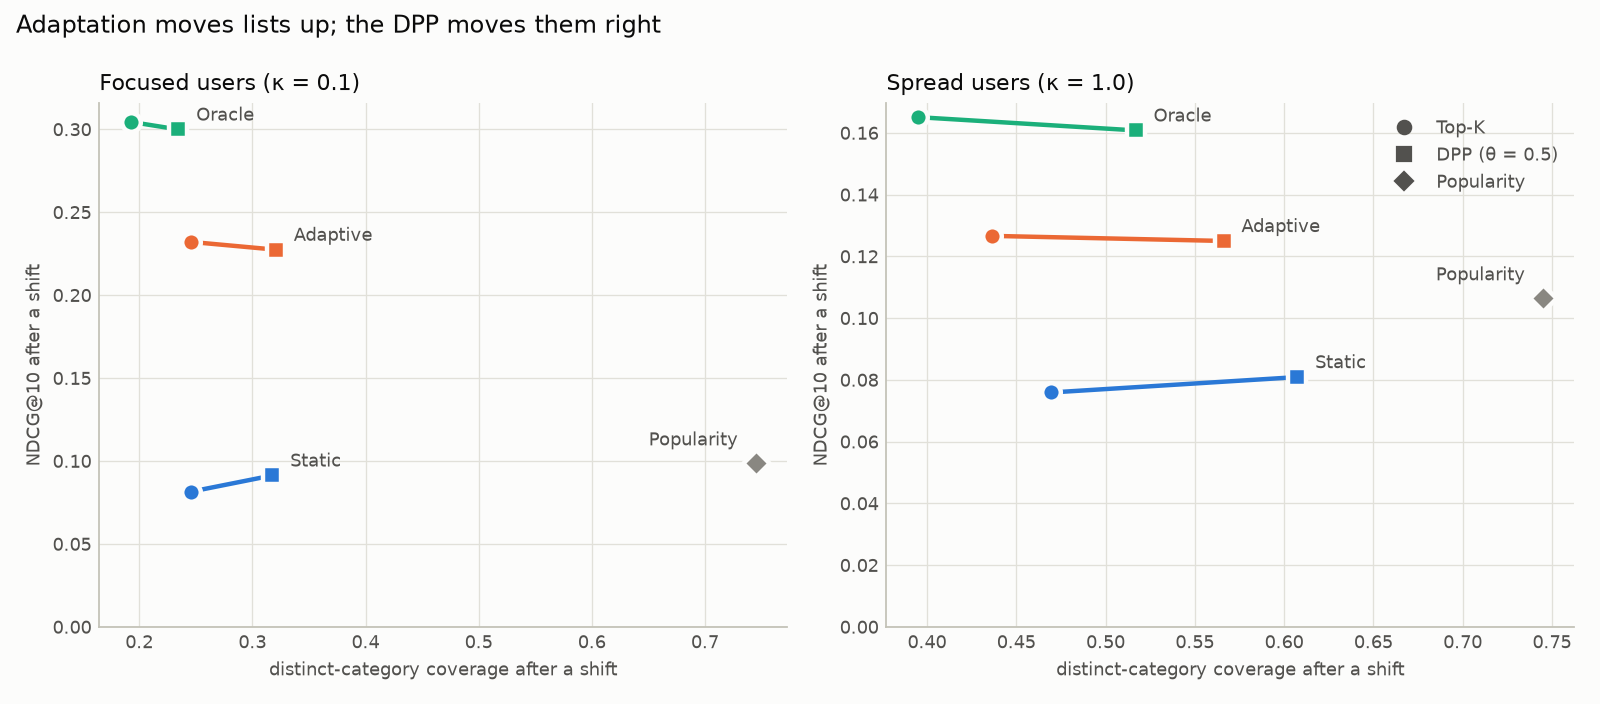
\includegraphics[width=\linewidth]{m8_tradeoff.png}
\caption[Relevance--coverage trade-off (M8)]{Post-shift NDCG against coverage. Arrows go from each Top-$K$ (circle) to its DPP
(square). \confirmatory\ \src{results/m9_analysis/20261102-151914/tradeoff.png}}
\label{fig:tradeoff}
\vspace{1em}
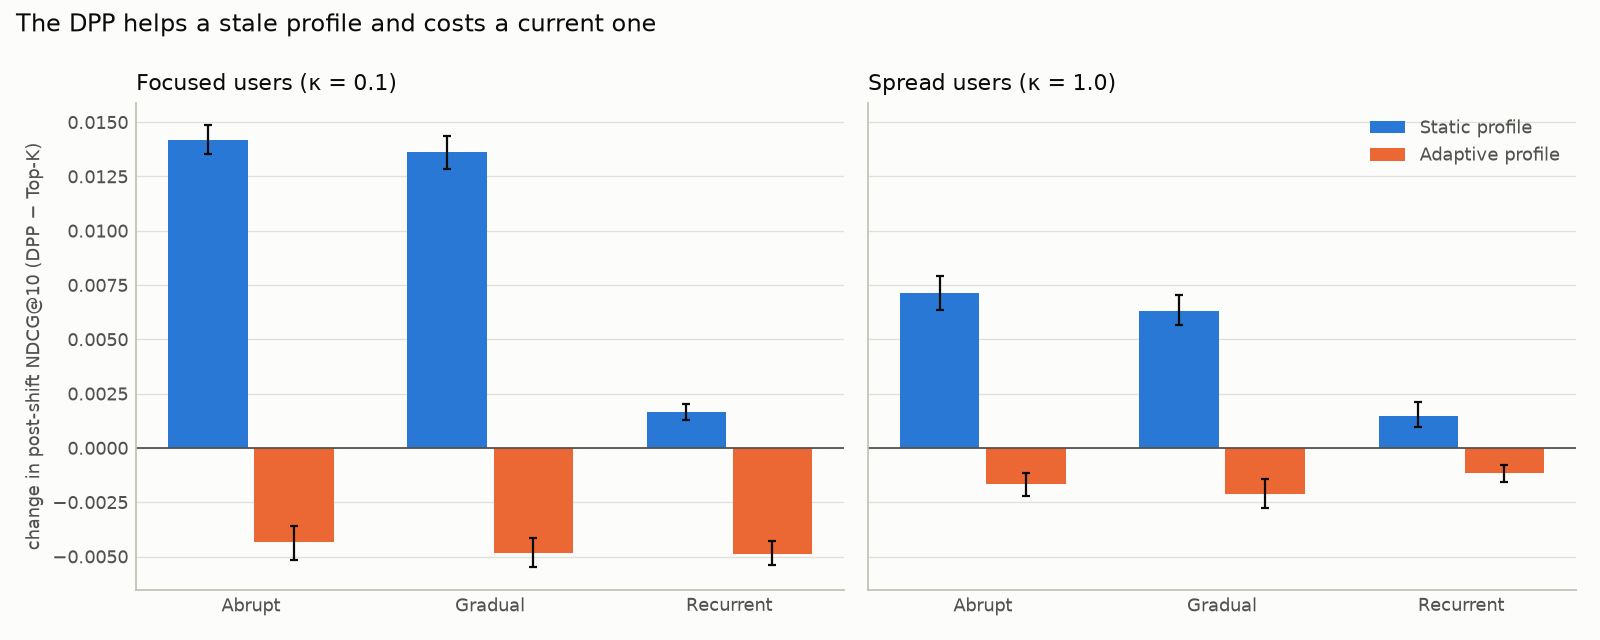
\includegraphics[width=\linewidth]{m8_dpp_effect.png}
\caption{DPP $-$ Top-$K$ on post-shift NDCG per drift scenario, with paired 95\% CIs. Positive
for the static profile in all 6 cells ($+0.0015$ to $+0.0142$), negative for the adaptive
profile in all 6 ($-0.0011$ to $-0.0049$). \confirmatory\ (descriptive breakdown)}
\label{fig:dppeffect}
\end{figure}

\begin{figure}[t]\centering
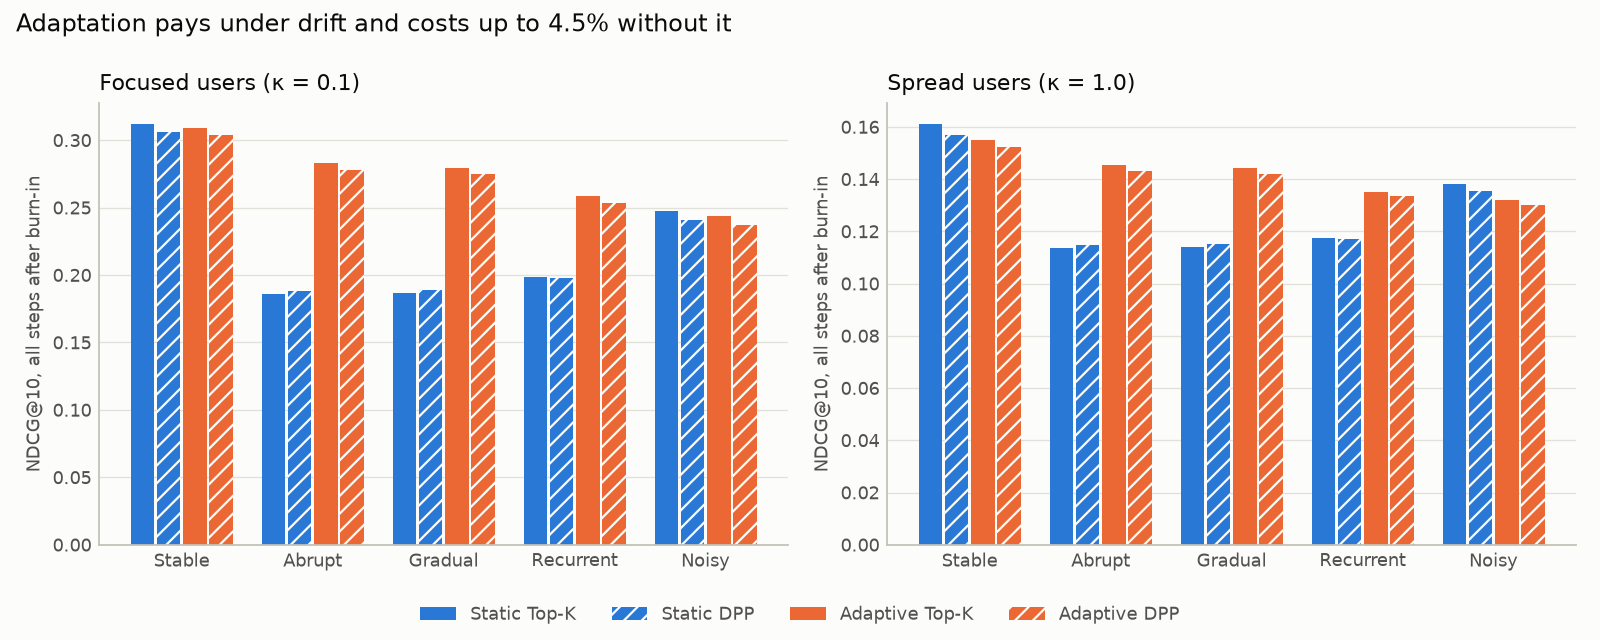
\includegraphics[width=\linewidth]{m8_scenario_ndcg.png}
\caption{Overall NDCG of the four factorial methods per scenario; hatching marks the DPP.
\confirmatory\ (descriptive breakdown)}
\label{fig:scenario}
\end{figure}

%=====================================================================================
\section{Analysis and exploratory follow-ups (Milestone 9)}\label{sec:m9}
%=====================================================================================

\subsection{Per-scenario breakdown of the confirmatory run}
Descriptive, outside Holm, from the saved records. \textbf{Pooling hid a per-cell cost.}
H4b meets the $\pm3\%$ rule pooled, but Adaptive Top-$K$'s overall NDCG is lower than Static
Top-$K$'s by:

\begin{table}[h]\centering\small
\begin{tabular}{lcc}
\toprule
 & Stable & Noisy \\
\midrule
Focused & $-0.8\%$ & $-1.4\%$ \\
Spread & $-3.7\%$ ($-0.0060$, CI [$-0.0064$, $-0.0054$]) & $-4.5\%$ ($-0.0062$, CI [$-0.0067$, $-0.0058$]) \\
\bottomrule
\end{tabular}
\end{table}
The frozen H4b verdict stands, and these cells should be reported beside it.

\subsection{$\alpha$ versus EWMA start}
\exploratory\ Seeds 200--219, 553\,s, \path{results/m9_alpha_start/20261102-151847/}. A $2\times2$
of $\alpha\in\{0.05,0.07\}$ and start $\in\{$bias-corrected, uniform$\}$:

\begin{table}[h]\centering\small
\begin{tabular}{lcc}
\toprule
Top-$K$ & $\alpha$ 0.07 $-$ 0.05 & Uniform $-$ bias-corrected start \\
\midrule
Post-shift NDCG & $+0.0114$ [0.0112, 0.0116] & $+0.00002$ [0.00001, 0.00002] \\
Post-shift coverage & $-0.0225$ [$-0.0235$, $-0.0215$] & $+0.0003$ \\
Stable NDCG & $-0.0024$ [$-0.0025$, $-0.0023$] & $+0.00002$ \\
All-scenario NDCG & $+0.0008$ [0.0007, 0.0009] & $+0.00002$ \\
\bottomrule
\end{tabular}
\end{table}
The ablation's gain came from $\alpha$, not from the start: the start's leftover weight
$(1-\alpha)^t$ is under 3\% by the first shift. A larger $\alpha$ helps after shifts and costs
when interests are stable, so neither value dominates. The frozen $\alpha=0.05$ stays.

\subsection{Sensitivity to $\theta$ and click noise $\eta$}
\exploratory\ Seeds 200--219, 1{,}614\,s, \path{results/m9_sensitivity/20261102-164513/}. Here
$\eta$ also changes the training population, and the noisy scenario runs only at the default
$\eta$. These sweep runs reproduce the $\alpha$ study's values exactly where they overlap
(5{,}120 of 5{,}120). CIs are not corrected for multiplicity.

\begin{table}[h]\centering\small
\begin{tabular}{ccccccc}
\toprule
$\theta$ & DPP effect, static & DPP effect, adaptive & Interaction (95\% CI) & Adaptive cov.\ gain & Adaptive EU loss \\
\midrule
0.9 & $+0.0010$ & $+0.0000$ & $-0.0010$ [$-0.0011$, $-0.0009$] & $+0.013$ & 0.03\% \\
0.7 & $+0.0036$ & $-0.0006$ & $-0.0042$ [$-0.0045$, $-0.0039$] & $+0.046$ & 0.62\% \\
0.5 & $+0.0073$ & $-0.0033$ & $-0.0105$ [$-0.0111$, $-0.0100$] & $+0.098$ & 3.12\% \\
0.3 & $+0.0118$ & $-0.0120$ & $-0.0238$ [$-0.0245$, $-0.0231$] & $+0.185$ & 10.84\% \\
\bottomrule
\end{tabular}
\caption{$\theta$ sweep at $\eta=0.05$: post-shift NDCG, drift pooled, both $\kappa$.}
\end{table}

\begin{table}[h]\centering\small
\begin{tabular}{cccccc}
\toprule
$\eta$ & Adaptation gain (post NDCG) & Stable cost, all & Focused & Spread & Interaction (95\% CI) \\
\midrule
0    & $+0.1079$ & $-1.59\%$ & $-0.64\%$ & $-3.43\%$ & $-0.0110$ [$-0.0115$, $-0.0105$] \\
0.05 & $+0.1003$ & $-1.68\%$ & $-0.69\%$ & $-3.58\%$ & $-0.0105$ [$-0.0111$, $-0.0100$] \\
0.15 & $+0.0861$ & $-1.92\%$ & $-0.83\%$ & $-3.95\%$ & $-0.0099$ [$-0.0105$, $-0.0093$] \\
0.3  & $+0.0648$ & $-2.51\%$ & $-1.26\%$ & $-4.73\%$ & $-0.0087$ [$-0.0094$, $-0.0081$] \\
\bottomrule
\end{tabular}
\caption{$\eta$ sweep: adaptation columns use Top-$K$, the interaction uses $\theta=0.5$.}
\end{table}

\paragraph{Findings.}
\begin{itemize}
  \item \textbf{Substitution is robust}: negative, with the CI excluding zero, at every $\theta$
        and $\eta$ tested and in both $\kappa$ groups. It grows with DPP strength and shrinks a
        little with noise.
  \item \textbf{The DPP cannot replace adaptation.} Its largest static gain is 0.0118, against
        0.1003 from adaptation; Static DPP at $\theta=0.3$ (0.0935) stays far below Adaptive
        Top-$K$ (0.1819).
  \item \textbf{Diversity gets expensive quickly}: for the adaptive profile, $\theta=0.7$ costs
        0.33\% of post-shift NDCG for $+0.046$ coverage, while $\theta=0.3$ costs 6.6\% for
        $+0.185$. For spread users at $\theta=0.7$ the cost is $-0.0001$ [$-0.0003$, $+0.0001$].
  \item \textbf{Adaptation survives noise.} Its gain falls about 40\% from $\eta=0$ to $0.3$
        and stays large. Spread users exceed a 3\% stable cost at every $\eta$, even
        $\eta=0$, so that cost is not caused by noise alone.
  \item Static post-shift NDCG rises slightly with $\eta$ (0.0803 to 0.0880). A plausible
        explanation, untested: noise flattens the target clicks, so a stale list misses
        slightly less.
\end{itemize}
\textbf{$\theta=0.7$ looks attractive here, but it was seen after the fact.} D-29 fixed the
rule in advance, so changing $\theta$ would need confirmation on fresh seeds.

\begin{figure}[p]\centering
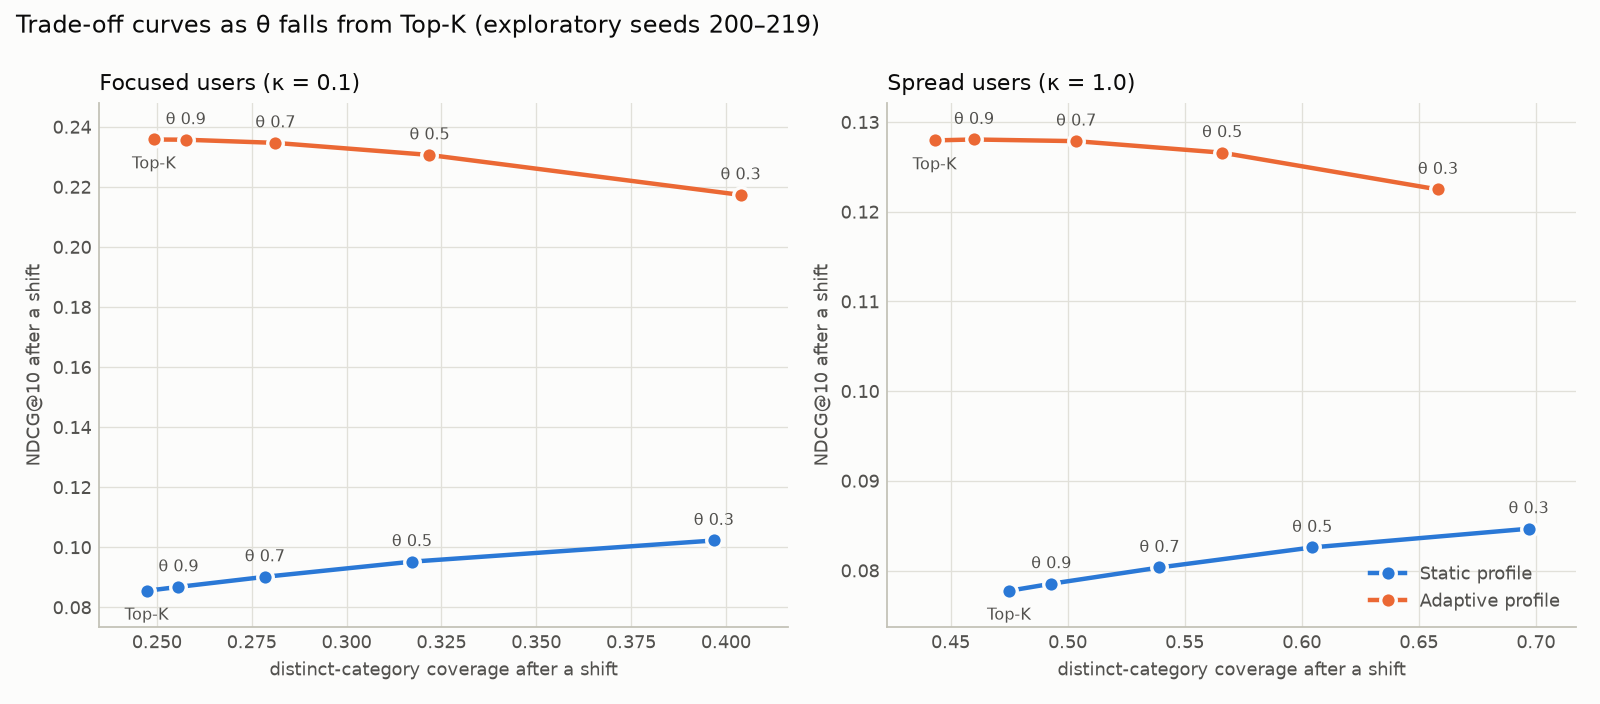
\includegraphics[width=\linewidth]{m9_frontier.png}
\caption[Trade-off curves along the theta sweep]{Post-shift NDCG against coverage as $\theta$ falls from Top-$K$, per profile and
concentration. \exploratory\ \src{results/m9_sensitivity/20261102-164513/frontier.png}}
\label{fig:frontier}
\vspace{1em}
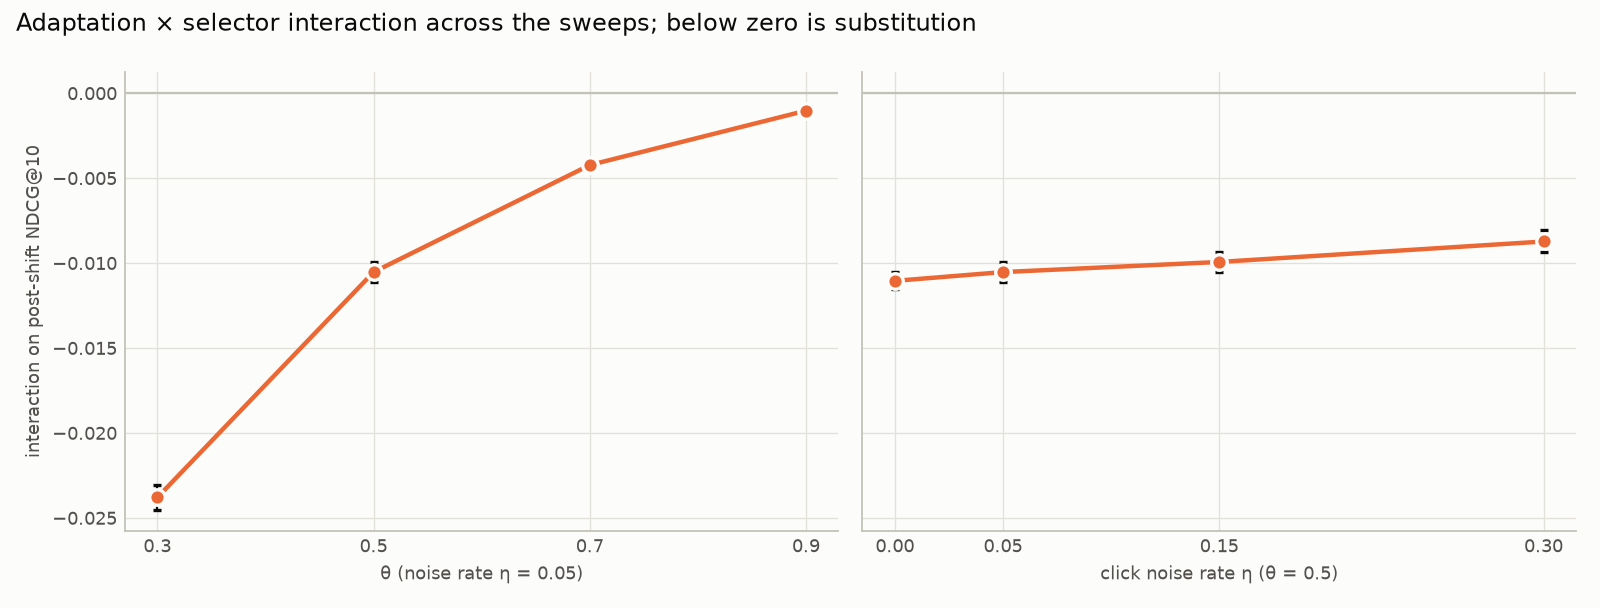
\includegraphics[width=\linewidth]{m9_interaction.png}
\caption{Adaptation $\times$ selector interaction with 95\% CIs along the $\theta$ and $\eta$
sweeps; below zero is substitution. \exploratory}
\label{fig:interaction}
\end{figure}

%=====================================================================================
\section{Calibration baseline (Milestone 10, D-19)}\label{sec:calib}
%=====================================================================================
\exploratory\ Planned since Milestone 1 to answer ``is a DPP needed at all?'', built after the
Steck paper was read in full. Code: \path{adaptdiv/calibration.py}.

\paragraph{Method} (after \citet{steck2018calibrated}, Eq.~6, with our adaptations). For the
method's own profile $p=\zhat_t$ and list $R$ with category mix $q_R$:
\begin{equation}
R_t=\arg\max_{|R|=K}\,(1-\lambda)\sum_{i\in R}\log s_i-\lambda\,\mathrm{KL}\big(p\,\|\,\tilde q_R\big),\qquad
\tilde q_R=(1-a)\,q_R+a\,p,\ a=0.01,
\end{equation}
built greedily one item at a time. $\lambda=0$ is Top-$K$. Adaptations: $\log s_i$ instead of
$s_i$ (the paper allows a monotone transform), no rank weights and no diversity prior (as in the
paper's experiments). Steck's own target allows recency weights (his Eq.~2), so an EWMA target is
within his framework. New descriptive metric for every method: miscalibration
$\mathrm{KL}(z_{t+1}\,\|\,\tilde q_R)$ against the \emph{true} interest.

\paragraph{Choosing $\lambda$} \tuning\ The same rule as $\theta$: the most calibrating
$\lambda$ with EU loss $\le3\%$ for both profiles
(\path{results/m10_calibration_lambda/20261103-160304/}).

\begin{table}[h]\centering\small
\begin{tabular}{lccccccc}
\toprule
$\lambda$ & 0.5 & \textbf{0.8} & 0.9 & 0.95 & 0.98 & 0.99 & 0.995 \\
\midrule
Static EU loss & $-0.5\%$ & 0.6\% & 2.6\% & 5.0\% & 7.3\% & 8.3\% & 8.9\% \\
Adaptive EU loss & 0.4\% & \textbf{2.8\%} & 5.6\% & 8.3\% & 10.5\% & 11.4\% & 12.0\% \\
\bottomrule
\end{tabular}
\caption{$\lambda=0.8$ selected; like $\theta$, it sits close to the limit.}
\end{table}

\paragraph{Comparison} \exploratory\ Seeds 200--219, 324\,s,
\path{results/m10_calibration/20261103-160313/}. Overall EU is equal for the two adaptive
diversifiers (0.2405 and 0.2405), so this compares them at a matched relevance budget. The DPP and
Top-$K$ values reproduce the sensitivity run exactly (10{,}240 of 10{,}240).

\begin{table}[h]\centering\small
\begin{tabular}{lccccc}
\toprule
Calibrated $-$ DPP & Post NDCG & Post coverage & Overall coverage & Miscalibration & ILD (abs.) \\
\midrule
Static & $+0.0027$ [0.0023, 0.0032] & $+0.107$ & $+0.091$ & $-0.283$ & 0.857 vs 0.845 \\
Adaptive & $-0.0000$ [$-0.0003$, 0.0003] & $+0.098$ & $+0.083$ & $-0.222$ & 0.840 vs 0.828 \\
\bottomrule
\end{tabular}
\caption{Pooled over $\kappa$; the same direction holds in both $\kappa$ groups.}
\end{table}

\noindent Interaction (adaptation $\times$ selector) on post-shift NDCG: DPP $-0.0105$
[$-0.0111$, $-0.0100$]; calibrated $-0.0133$ [$-0.0137$, $-0.0128$].

\paragraph{Findings.}
\begin{itemize}
  \item \textbf{At the same relevance budget, the DPP added nothing that calibration did not.}
        With the adaptive profile NDCG and EU tie, and calibration gives about 0.08--0.10 more
        coverage, lower miscalibration and even slightly higher ILD, the measure the DPP optimises.
  \item By H6a's rule Adaptive Calibrated does not formally dominate Adaptive DPP, only because
        NDCG is tied.
  \item \textbf{Substitution is not DPP-specific.} Calibration shows it too, slightly more strongly.
  \item A plausible reason, untested: embeddings are clustered by category (cross-category cosine
        about 0), so embedding diversity is mostly category diversity, which calibration targets
        directly. A catalogue with real within-category variety might favour a DPP; this
        simulator cannot show it.
\end{itemize}

\begin{figure}[h]\centering
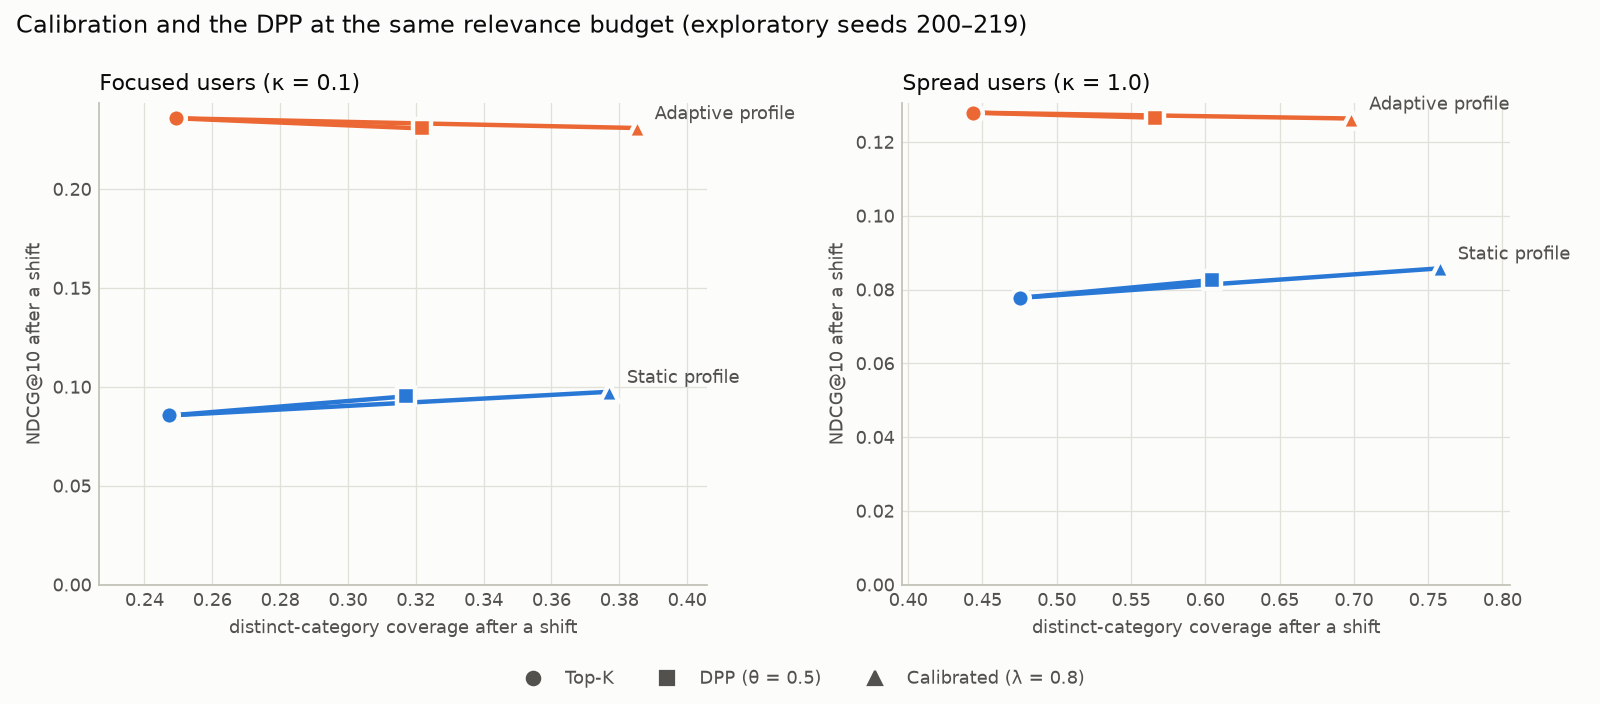
\includegraphics[width=\linewidth]{m10_calibration_tradeoff.png}
\caption[Calibration vs DPP trade-off]{Post-shift NDCG against coverage for Top-$K$ (circle), DPP $\theta=0.5$ (square)
and calibrated $\lambda=0.8$ (triangle). \exploratory\
\src{results/m10_calibration/20261103-160313/calibration_tradeoff.png}}
\label{fig:calib}
\end{figure}

%=====================================================================================
\section{Negative results}\label{sec:negative}
%=====================================================================================
\begin{itemize}
  \item Diversification did not help the adaptive profile's relevance: the interaction is
        substitution, not complementarity, at every $\theta$ and $\eta$ tested.
  \item The proposed configuration is not the best adaptive setting for post-shift NDCG:
        $\alpha=0.07$ is about 6\% higher, though it costs stable NDCG and coverage.
  \item Adaptive DPP's out-of-sample EU loss (3.04\%) exceeded the 3\% limit met on tuning seeds.
  \item Adaptation has real costs: worse stable tracking (H2), more false switches (H3), and
        lower stable NDCG, up to 3.7--4.7\% for spread users.
  \item After a shift, the static profile is worse than plain Popularity.
  \item $\theta=0.3$ costs the adaptive profile about 6.6\% post-shift NDCG and 10.8\% EU.
  \item At a matched relevance budget the DPP was no better than a calibrated re-ranker, which gave
        more coverage, lower miscalibration and slightly higher ILD (\S\ref{sec:calib}).
\end{itemize}

%=====================================================================================
\section{Limitations and threats to validity}\label{sec:limits}
%=====================================================================================
\begin{enumerate}
  \item \textbf{Synthetic only.} The generator is category-driven and the scorer is
        category-weighted, which favours category-level profiles. Mitigations: a hidden taste
        $\lambda>0$, a stable scenario where adaptation should not help, two $\kappa$ levels,
        and a noise sweep.
  \item \textbf{Open loop.} Recommendations never change behaviour, so there is no feedback
        loop and no exposure effect.
  \item \textbf{Repeats allowed.} 69--87\% of Top-$K$ list items were already clicked (tuning
        check), and repeats are 33--64\% of targets. The results apply to domains with repeat
        consumption, and new-item metrics are a sensitivity check.
  \item \textbf{Fixed shift times} and a half-swap shift; no randomised $\tau$. A pooled
        tuning mix with 2 of 5 scenarios without drift shapes $\alpha$.
  \item \textbf{Adapted DPP objective} (log form), so Chen et al.'s results do not transfer;
        greedy quality is verified on tiny instances only.
  \item \textbf{$\theta$ near the rule limit} (2.8\% on tuning, 3.04\% out of sample).
  \item \textbf{Censored lags} understate H1a.
  \item \textbf{Noise floor}: estimators track $(1-\eta)z+\eta/C$, not $z$.
  \item \textbf{Narrow CIs} reflect variation between 20 paired seeds with shared randomness,
        not generalisation. Exploratory CIs are uncorrected.
  \item \textbf{Exploratory follow-ups} were chosen after seeing confirmatory results, and seeds
        200--219 are shared across the follow-up studies.
  \item \textbf{Calibration baseline is exploratory}: added after the confirmatory run, on seeds
        200--219; $\lambda$'s grid has no value between 0.8 and 0.9.
  \item \textbf{Literature} mostly verified at metadata or abstract level; targeted search.
\end{enumerate}

%=====================================================================================
\section{Pending items}\label{sec:pending}
%=====================================================================================
\begin{itemize}
  \item Done on 3 November 2026: the calibration baseline (D-19), \S\ref{sec:calib}.
  \item \pending\ Deadline (D-07) not recorded.
  \item Not done by design: real-data validation (D-31); a randomised shift-time sensitivity check;
        $\lambda$ and $\kappa=0.3$ sensitivity.
\end{itemize}

%=====================================================================================
\section{Reproducibility}\label{sec:repro}
%=====================================================================================
Repository \url{https://github.com/Shambo-Roy/ire-adaptive-dpp-rec}. Python 3.12.10, NumPy
2.5.2, SciPy 1.18.0, matplotlib 3.11.1; CPU only (Windows 11, 20 logical CPUs). The test suite
has 188 tests (\texttt{python -m pytest -q}).

\begin{table}[h]\centering\small
\begin{tabularx}{\linewidth}{lXl}
\toprule
Milestone & Command & Output \\
\midrule
M3 & \texttt{python experiments/sim\_check.py} & \path{results/m3_sim_check/} \\
M4 & \texttt{python experiments/estimator\_study.py}; \texttt{ewma\_init\_comparison.py} & \path{results/m4_*} \\
M5 & \texttt{python experiments/relevance\_check.py} & \path{results/m5_relevance/} \\
M6 & \texttt{python experiments/dpp\_check.py} & \path{results/m6_dpp/} \\
M7 & \texttt{python experiments/select\_theta.py} & \path{results/m7_theta/} \\
M8 & \texttt{python experiments/main\_experiment.py} (about 14 min) & \path{results/m8_main/} \\
M9 & \texttt{python experiments/m9\_figures.py} & \path{results/m9_analysis/} \\
M9 & \texttt{python experiments/alpha\_start\_study.py} (about 9 min) & \path{results/m9_alpha_start/} \\
M9 & \texttt{python experiments/sensitivity\_study.py} (about 27 min); \texttt{sensitivity\_figures.py} & \path{results/m9_sensitivity/} \\
M10 & \texttt{python experiments/select\_calibration.py} (about 2 min) & \path{results/m10_calibration_lambda/} \\
M10 & \texttt{python experiments/calibration\_study.py --lam 0.8} (about 5.5 min); \texttt{calibration\_figures.py} & \path{results/m10_calibration/} \\
\bottomrule
\end{tabularx}
\end{table}
Every run folder stores \texttt{config.json}, the seed list, NumPy version, git HEAD and
status, and its runtime. The main experiment refuses to run if \path{adaptdiv/} differs from
HEAD.

%=====================================================================================
\section{Claim-to-evidence map}\label{sec:map}
%=====================================================================================
\begin{table}[h]\centering\small
\begin{tabularx}{\linewidth}{Xl}
\toprule
Claim & Evidence \\
\midrule
EWMA recovers faster and tracks better after drift & H1a, H1b; estimation table (\S\ref{sec:m8}) \\
Adaptation costs accuracy when stable or noisy & H2, H3, H4b; per-scenario table (\S\ref{sec:m9}) \\
Adaptation raises post-shift relevance a lot & H4a; Table~\ref{tab:pooled}; Fig.~\ref{fig:tradeoff} \\
The DPP raises coverage at a small relevance cost & H5a; Table~\ref{tab:pooled}; Fig.~\ref{fig:frontier} \\
The DPP's cost is slightly larger for focused users & H5b (very small) \\
Adaptation and DPP substitute & H6b; Fig.~\ref{fig:dppeffect}; Fig.~\ref{fig:interaction} \\
Adaptive DPP is not dominated & H6a \\
The DPP adds nothing over calibration here & \S\ref{sec:calib}; Fig.~\ref{fig:calib} \\
The $\alpha=0.07$ ablation gain comes from $\alpha$ & \S\ref{sec:m9}, $\alpha$ $\times$ start \\
Estimation matters more than selection & Oracle gap 0.055 vs DPP cost 0.0032 \\
\bottomrule
\end{tabularx}
\end{table}

\appendix
%=====================================================================================
\section{Viva preparation}\label{sec:viva}
%=====================================================================================

\subsection*{Design}
\begin{description}[style=nextline]
  \item[Why a simulation and not a real dataset?] Real logs do not reveal the true interest
        $z_t$ or when it changed. Without them we cannot measure tracking error, lag or false
        switches, and cannot separate estimation from selection. The price is external validity.
  \item[Doesn't the simulator favour your method?] Partly: generator and scorer are both
        category-based. Mitigations: hidden taste the recommender cannot model, a stable
        scenario where adaptation should lose (it did, H2 and H4b), a noisy scenario, and
        reporting every scenario. The oracle still misses, because of $\lambda>0$.
  \item[Why open-loop?] To isolate estimation and selection effects. Closed-loop feedback
        would mix them with exposure effects. It is a stated limitation.
  \item[Why a half-swap shift?] It keeps concentration constant, so drift is not confounded
        with a change in how focused the user is. A top-2 swap was too weak for spread users
        (mean TV 0.36).
  \item[Why common random numbers?] Scenario differences then come only from the trajectory,
        and comparisons are paired, which lowers variance.
  \item[Why not a neural session model?] The question is about the profile and the selector.
        A transparent plug-in scorer keeps the effects interpretable, and simple models are
        often competitive \citep{ludewig2018evaluation}.
\end{description}

\subsection*{Estimation}
\begin{description}[style=nextline]
  \item[Why bias-corrected EWMA?] With a uniform start, the stable-scenario gap mixed two
        causes: forgetting and the prior. Bias correction removes the prior. It also shifted
        tuning from $\alpha=0.07$ to $0.05$.
  \item[What is the EWMA's mean memory?] Mean observation age $(1-\alpha)/\alpha=19$ steps at
        $\alpha=0.05$. A window with the same mean age has $W\approx2/\alpha-1=39$.
  \item[Why does EWMA beat a window at matched memory?] EWMA weights the newest observations
        most, so it crosses over sooner: 9.3 steps for EWMA(0.07) against 13.5 for a window of the same mean age (28), on tuning seeds.
  \item[Why is H1a's 67 steps an underestimate?] The cumulative mean never crosses over within
        the horizon for 64\% of abrupt and gradual cases; those lags are recorded at the horizon.
  \item[Should you switch to $\alpha=0.07$?] Not on this evidence. It gains about 6\% after
        shifts and loses when stable. The right value depends on how often interests change, and
        it would need confirming on fresh seeds.
\end{description}

\subsection*{DPP}
\begin{description}[style=nextline]
  \item[What does $\det S_Y$ measure?] The squared volume spanned by the selected embeddings.
        Near-duplicates make it small, so the determinant rewards spread.
  \item[Why greedy and not exact MAP?] Exact MAP is NP-hard. Greedy with Chen et al.'s updates
        costs $O(K^2N)$, about 0.15\,ms per list, and found the exact optimum in 95--100\% of
        tiny tests.
  \item[Why your own objective form?] Chen's linear form ignored relevance at our score scale.
        The log form makes $\theta=1$ exactly Top-$K$ and is still a valid DPP.
  \item[Why sort DPP lists before NDCG?] The DPP picks a set. Greedy order is an artefact that
        cost up to 0.9\% NDCG in a probe, and sorting gives both selectors the same ranking rule.
  \item[Why coverage and not ILD as the diversity metric?] The DPP optimises embedding
        similarity directly, so ILD gains are partly true by construction.
  \item[How was $\theta$ chosen?] Before evaluation, on tuning seeds: the most diverse $\theta$
        whose EU loss was at most 3\% for both profiles.
\end{description}

\subsection*{Results}
\begin{description}[style=nextline]
  \item[What does substitution mean?] The DPP helps less when the profile is already current.
        It helps a stale profile by hedging, since diversity spreads slots onto categories the
        user may have moved to. It costs a current profile relevance.
  \item[So is the DPP useless?] No. It buys coverage for a small relevance cost, but it does
        not improve relevance for a current profile, and it cannot replace adaptation (0.0118 vs
        0.1003).
  \item[Why does the static profile lose to Popularity after a shift?] It still recommends the
        old categories, which the user has left. Popularity at least spreads across categories.
  \item[Why does the static DPP's EU rise while the adaptive DPP's falls?] A list built on wrong
        weights has room to improve. A list built on nearly right weights can only give up
        relevance.
  \item[Why are the confidence intervals so narrow?] They cover 20 paired seeds with shared
        randomness and 100 users per cell. They describe seed variability in this simulator, not
        generalisation.
  \item[Why seed-level tests and not user-level?] Users within a seed share a catalogue and are
        not independent. The seed is the unit that is replicated.
  \item[Why does H4b pass while spread users lose 3.7--4.5\%?] H4b was frozen as a pooled test.
        The per-cell breakdown is descriptive and reported beside it rather than replacing it.
  \item[Why use new seeds for follow-ups?] The follow-up questions came from looking at
        evaluation results. Answering them on the same seeds would mix discovery with
        confirmation.
  \item[Did you compare against a non-DPP diversifier?] Yes, a calibrated re-ranker after Steck,
        chosen by the same EU rule. At equal relevance it beat the DPP on coverage, miscalibration and
        even ILD. In this simulator the DPP is not needed for these goals; it might matter where
        items vary within categories.
  \item[Why $\lambda=0.8$ and not Steck's 0.99?] Our score term is a sum of log scores over 10 items
        and 10 categories, so the scales differ. $\lambda$ was chosen by the same rule as $\theta$.
  \item[What would you do next?] Real logs with proxy drift labels; a
        closed-loop simulator; adaptive-rate estimators such as ADWIN \citep{bifet2007adwin};
        randomised shift times.
\end{description}

\subsection*{Key numbers to remember}
\begin{itemize}
  \item Adaptation: $+0.101$ post-shift NDCG ($+131\%$); lag gap $+67$ steps; TV gap $0.248$.
  \item Cost of adaptation: stable TV $+0.045$; false switches 0.074 vs 0.017 in the noisy
        scenario; stable NDCG about $-1.8\%$.
  \item DPP: coverage $+0.089$; NDCG cost 1.8\%; EU loss 3.04\%.
  \item Interaction: $-0.0106$ (substitution). Oracle gap: 0.055.
  \item Calibration vs DPP (adaptive, equal EU): NDCG tie, coverage $+0.083$ overall.
  \item Scale: 20 evaluation seeds $\times$ 2 $\kappa$ $\times$ 5 scenarios $\times$ 100 users
        $\times$ 200 steps.
\end{itemize}

\bibliographystyle{plainnat}
\bibliography{references}

\end{document}
